\chapter{Der \glqq ideale\grqq{} Dev(Sec)Ops Prozess}

Bereits im letzten Abschnitt wurde klar: Jeder kann sich Elemente der DevOps-Kultur aneignen und nach belieben kombinieren. 
Eine \glqq Musterlösung\grqq{} für den idealen Prozess kann es also nicht geben. 

Trotzdem gibt es Anordnungen der CI/CD/CT-Pipeline, die Vorteile gegenüber anderen Anordnungen mit sich bringen. 

In diesem Kapitel soll eine Pipeline beispielhaft modelliert und nach einer persönlichen Einschätzung hin optimiert werden.

\section{Welche Werkzeuge kommen zum Einsatz?}

Die Zahl der CI/CD-Werkzeuge, die bei der Konstruktion einer Pipeline zur Verfügung stehen ist groß \cite{xebialabsXebiaLabsPrasentiertPeriodensystem2018} \cite{digital.aiPeriodicTableDevOps}. Würde man versuchen jedes Werkzeug zu integrieren / zu behandeln, so könnte man keinem gerecht werden.
Aus diesem Grund soll an dieser Stelle eine Auswahl an Werkzeugen behandelt werden. Diese setzt sich zusammen aus den Werkzeugen die im Seminar behandelt wurden, Teil von Vorträgen waren oder vom Autor als wichtig erachtet werden.

Die folgenden Abschnitte bieten eine Übersicht über die betrachteten Werkzeuge:

\subsection{Abschnitt: Continuous-Integration}
Coding Style Guidelines (Bei uns: Arch Unit)
Code Architecture (Bei uns: Arch Unit)
Commit-Conventions (z.B. kurze GitLab Skripts)
(Pre-) Versioning (z.B. kurze GitLab Skripts)
License-Checker (Bei uns: GitLab)

\subsection{Abschnitt: Continuous-Testing}
Unit-Tests (z.B. jUnit, phpUnit)
Vulnerability-Checker (Bei uns: Snyk)
E2E-Tests (z.B. Selenium)
Dynamic Application Security Testing (DAST) (Automatisierte Pentests, Bei uns: GitLab)

Application Security Management; Test / Code coverage (Aggregiert Infos aus allen Quellen, Weniger Tool, mehr Auswertung)

\subsection{Abschnitt: Continuous-Delivery}
Application Building (z.B. GitLab Skripts zum kompilieren für verschiedene Systeme)
Application Deployment (z.B. GitLab Skripts zum deploy; Zero Downtime Deployments oder zumindest Wartungsmodus)
Application Monitoring (Bei uns: Sentry)


\section{Wie ordnet man seine Pipeline am besten an?}

Nicht nur die Wahl der Werkzeuge ist entscheidend, sondern auch die Reihenfolge der Anordnung \cite{nemytchenkoGitLabCIRun2016}. 
Sinnvolle Priorisierung und Parallelisierung können die Feedback-Zeit verringern und die Server entlasten. 

\begin{figure}[p]
    \vspace*{1cm}
    \setlength{\abovecaptionskip}{10pt}
    \setlength{\belowcaptionskip}{0pt}
    \centering
    \makebox[\textwidth][c]{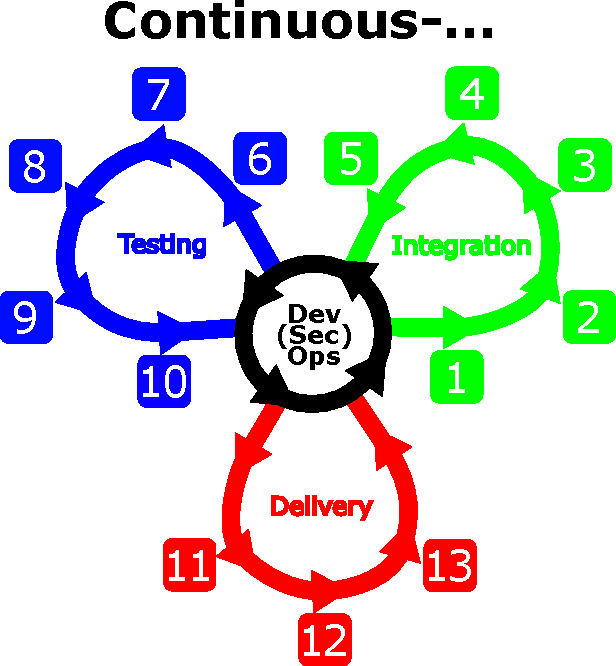
\includegraphics[width=\textwidth]{cicd_process.pdf}}
    \caption{Grafische Darstellung des \glqq idealen\grqq{} Dev(Sec)Ops Prozesses in Form einer CI/CT/CD-Pipeline. 
    Die drei Arme stellen die drei Phasen (Integration, Testing und Delivery) dar. Die Pfeile geben dabei die Richtung und den Weg an, in dem eine Änderung in die Produktionsumgebung über gehen kann. 
    Die Zahlen entsprechen dabei mit ihrer Nummerierung den Werkzeugen, wie sie in der Pipeline angeordnet werden. 
    Betont werden soll, dass über den inneren Kreis Stufen wiederholt werden können. Scheitert beispielsweise eine Änderung an einem Werkzeug in der \emph{Testing}-Phase, so wird die \emph{Delivery}-Phase innen übersprungen und mit der \emph{Integration}-Phase erneut begonnen. 
    Damit soll betont werden, dass Feedback von jedem Punkt schnell wieder zum Ausgangspunkt zurückfließen kann. }
    \label{fig:cicdprocess}
\end{figure}